\documentclass[tikz,border=5pt]{standalone}
\usepackage{ctex,amsmath}
\usetikzlibrary{arrows.meta,calc,decorations.pathmorphing}
\tikzset{>=Latex,body/.style={draw=black,thick,fill=blue!5},
 guide/.style={gray!65,dashed},vel/.style={blue!70!black,very thick,->},
 force/.style={orange!85!black,very thick,->}}
\newcommand{\wall}[2]{
 \draw[very thick](#1,#2-.25)--(#1,#2+1.2);
 \foreach \dy in {-.2,0,.2,.4,.6,.8,1.0}{
  \draw[gray!65](#1,#2+\dy)--(#1+.18,#2+\dy+.14);}}
\newcommand{\spring}[3]{
 \draw[thick](#1,#3)--(#1+.15,#3);
 \draw[thick,decorate,decoration={zigzag,segment length=5pt,amplitude=3pt}]
  (#1+.15,#3)--(#2-.15,#3);
 \draw[thick](#2-.15,#3)--(#2,#3);}
\begin{document}
\begin{tikzpicture}[font=\large]
 \draw[thick](-.15,0)--(9.5,0);
 \path[body](.8,0)--(2.65,1.9)
  ..controls(2.82,2.06)and(2.91,2.09)..(3.005,2.09)
  ..controls(3.1,2.09)and(3.22,2.08)..(3.35,1.98)
  --(5.05,.15)..controls(5.18,.015)and(5.26,0)..(5.45,0)--cycle;
 \fill(3.005,2.09)circle(.055)node[above left]{$m$};
 \node at(3.05,.72){$M$};
 \draw[<->](.4,0)--(.4,2.09)node[midway,left]{$h$};
 \draw[guide](.4,2.09)--(2.86,2.09);
 \draw[vel](3.2,2.35)--(4.05,2.35)node[right]{微扰};
 \wall{9.2}{.25}
 \spring{8.15}{9.2}{.25}
 \draw[thick](8.15,.07)--(8.15,.43);
 \draw[gray!75](8.15,.43)--(8.15,.68)--(9.2,.68);
 \node[above]at(8.64,.72){细绳};
 \node[below]at(8.7,-.3){$k$};
 \draw[guide](7.45,.08)--(7.45,.85);
 \draw[<->](7.45,.93)--(8.15,.93)node[midway,above]{$x_0$};
\end{tikzpicture}
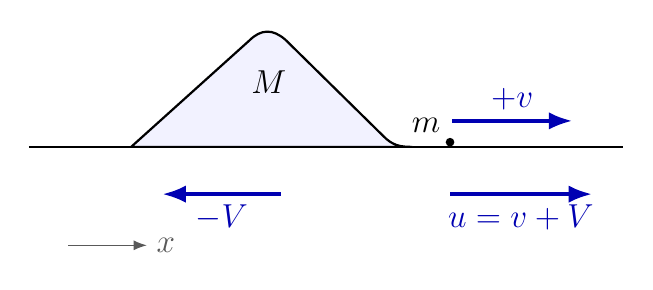
\begin{tikzpicture}[font=\large]
 \draw[thick](-.3,0)--(7.25,0);
 \path[body](1,0)--(2.5,1.35)
  ..controls(2.65,1.5)and(2.8,1.5)..(2.96,1.36)
  --(4.2,.14)..controls(4.32,.015)and(4.42,0)..(4.57,0)--cycle;
 \node at(2.75,.82){$M$};
 \draw[vel](2.9,-.6)--(1.4,-.6)node[midway,below]{$-V$};
 \fill(5.05,.06)circle(.055)node[above left]{$m$};
 \draw[vel](5.08,.33)--(6.6,.33)node[midway,above]{$+v$};
 \draw[vel](5.05,-.6)--(6.85,-.6)node[midway,below]{$u=v+V$};
 \draw[->,gray!70!black](.2,-1.25)--(1.2,-1.25)node[right]{$x$};
\end{tikzpicture}
\begin{tikzpicture}[font=\large]
 % 两幅状态使用同一个固定自然长原点和墙位置。
 \foreach \yy/\xx/\lab in {0/2.1/{初接触},-2.8/1.1/{分离}}{
  \begin{scope}[yshift=\yy cm]
   \wall{5.5}{.3}\spring{\xx}{5.5}{.3}
   \draw[thick](\xx,.20)--(\xx,.40);
   \fill(\xx,.3)circle(.06);
   \node[above]at(\xx,.44){$m$};
   \draw[guide](1.1,-.3)--(1.1,1.3);
   \node[below]at(1.1,-.32){$O_s:\ \xi=0$};
   \node[left]at(.1,.85){\lab};
  \end{scope}}
 \draw[<->](1.1,1.2)--(2.1,1.2)node[midway,above]{$\xi(0)=x_0$};
 \draw[vel](2.2,.8)--(3.45,.8)node[midway,above]{$+v$};
 \draw[force](2.05,.3)--(.35,.3);
 \node[above]at(.85,.38){$-k\xi$};
 \draw[vel](1.0,-1.85)--(.2,-1.85)node[midway,above]{$-w$};
 \draw[->,gray!70!black](3.6,-3.4)--(4.6,-3.4)node[right]{$+\xi$};
\end{tikzpicture}
\begin{tikzpicture}[font=\large]
 \begin{scope}
  \draw[thick](-.15,0)--(5.8,0);
  \path[body](.5,0)--(1.85,1.3)
   ..controls(2,1.44)and(2.14,1.44)..(2.3,1.3)
   --(3.57,.12)..controls(3.69,.015)and(3.79,0)..(3.9,0)--cycle;
  \node at(2.12,.87){$M$};
  \draw[vel](2.3,-.6)--(1.05,-.6)node[midway,below]{$-V$};
  \fill(4.9,.06)circle(.055)node[above right]{$m$};
  \draw[vel](4.9,.65)--(3.65,.65)node[midway,above]{$-w$};
  \draw[vel](4.9,-.6)--(3.4,-.6)node[midway,below]{$-(w-V)$};
  \node at(2.7,1.9){返回底部};
 \end{scope}
 \begin{scope}[xshift=7.2cm]
  \draw[thick](-.15,0)--(4.25,0);
  \path[body](.5,0)--(1.85,1.3)
   ..controls(1.95,1.4)and(2.0,1.405)..(2.075,1.405)
   ..controls(2.15,1.405)and(2.22,1.38)..(2.3,1.3)
   --(3.57,.12)..controls(3.69,.015)and(3.79,0)..(3.9,0)--cycle;
  \fill(2.075,1.405)circle(.055);
  \node[right]at(2.45,1.49){$m$};
  \node at(2.15,.6){$M$};
  \draw[<->](.1,0)--(.1,1.405)node[midway,left]{$h$};
  \draw[vel](2.25,1.75)--(.95,1.75)node[midway,above]{$V_C<0$};
  \node at(2.05,-.65){$v_m-v_M=0$};
  \node at(2.05,2.42){顶端临界};
 \end{scope}
\end{tikzpicture}
\begin{tikzpicture}[font=\large,x=1.5cm,y=2cm]
 \def\th{.55}
 \draw[->](-.1,0)--(4.1,0)node[right]{$\varphi=\omega t+\theta$};
 \draw[->](0,-.45)--(0,1.35)node[above]{$\xi/A$};
 \draw[gray!60,dashed,domain=0:.55,samples=30]plot(\x,{sin(deg(\x))});
 \draw[blue!70!black,very thick,domain=.55:pi,samples=100]plot(\x,{sin(deg(\x))});
 \draw[gray!60,dashed,domain=pi:3.55,samples=30]plot(\x,{sin(deg(\x))});
 \draw[guide](.55,0)--(.55,{sin(deg(.55))});
 \fill[blue!70!black](.55,{sin(deg(.55))})circle(.03);
 \node[above left]at(.55,{sin(deg(.55))}){$x_0/A$};
 \draw[guide](pi/2,0)--(pi/2,1)--(0,1);
 \fill[blue!70!black](pi/2,1)circle(.03)node[above]{最大压缩};
 \fill[blue!70!black](pi,0)circle(.03)node[above right]{分离};
 \node[left]at(0,1){$1$};
 \node[below]at(.55,0){$\theta$};
 \node[below]at(pi/2,0){$\pi/2$};
 \node[below]at(pi,0){$\pi$};
 \draw[<->](.55,-.65)--(pi,-.65)node[midway,below]{$\omega t_{\rm sep}=\pi-\theta$};
 \node[gray!70!black,right]at(3.48,-.42){数学延拓};
\end{tikzpicture}
\end{document}
